
\begin{figure}
\begin{subfigure}[b]{0.5\textwidth}
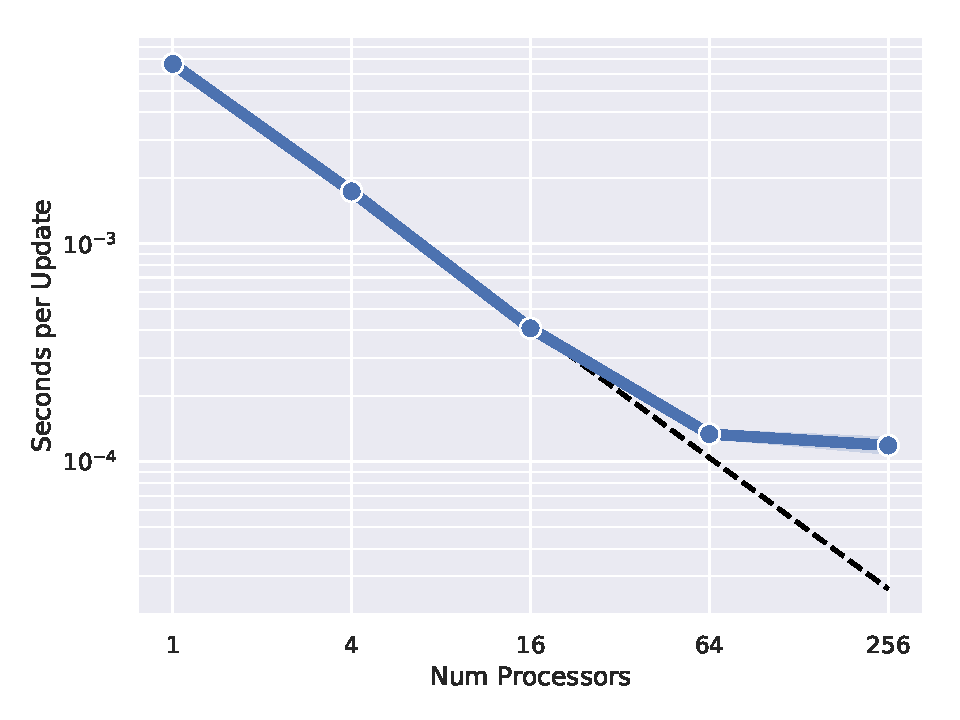
\includegraphics[width=\textwidth]{img/MPIStrong}
\caption{
MPI implementation
}
\label{fig:mpi_weak}
\end{subfigure}
\begin{subfigure}[b]{0.5\textwidth}
  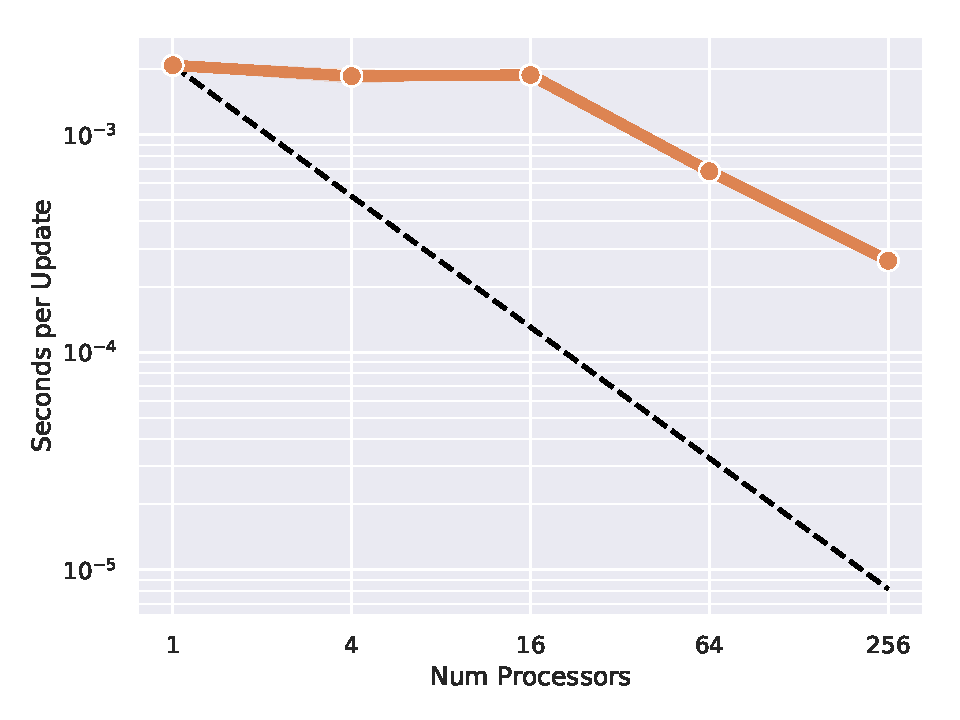
\includegraphics[width=\textwidth]{img/CharmStrong}
\caption{
Charm++ implementation
}
\label{fig:charm_weak}
\end{subfigure}
\caption{
Strong scaling analysis (time to solution versus parallelism for a fixed problem size) for MPI (\subref{fig:mpi_weak}) and Charm++ (\subref{fig:charm_weak}) implementations.
Dashed line indicates the ideal scaling relationship.
Shaded area represents standard deviation of five replications for each observation.
Fixed problem size was a $2048\times2048$ grid for the MPI implementation and a $16\times16$ grid for the Charm++ implementation.
}
\label{fig:weak}
\end{figure}
